\documentclass{article}
\usepackage{graphicx}
\usepackage{fvextra}
\usepackage{hyperref}
\usepackage{geometry}
 \geometry{
    a4paper,
    total={170mm,257mm},
    left=20mm,
    top=20mm,
}
\hypersetup{
    colorlinks=true,
    urlcolor=blue,
}

\def\gate#1{\uppercase{\Verb|#1|}}

\title{David's Universal Number Kounter}
\author{David Farrell}
\date{May 2025}

\begin{document}

\maketitle

\section{Introduction}

David's Universal Number Kounter, ``dunk", is a fully-16-bit micro-coded CPU designed in Logisim-evolution. Let me explain those terms. First, ``fully-16-bit'': everything in dunk has a 16-bit bit width. The registers, buses, instructions, and even memory cells in dunk are 16 bits in width. Memory is addressed in 16 bit words, rather than bytes; each memory address (themselves 16 bits) refers to a 16 bit word in main memory, and read and write operations only deal with these 16-bit words. This is for simplicity; this project was created as an educational exercise, and the broad design was established at a time where my knowledge of CPU architecture was more limited. By ``micro-coded'', I mean that every machine code instructions is translated on-the-fly by the control unit into a sequence of so-called ``micro-code instructions'' which instruct the various parts of the CPU on how to actually carry out the instructions. While a machine code instruction might be something like, ``load the value of memory at the address stored in register 1 into register 2", micro-code instructions are much more granular; for instance, the aforementioned instruction would be carried out by the sequence ``output the value of register 1 to the address bus; send the output of the memory unit to the data bus; write the content of the data bus to register 2". As for Logisim-evolution; \href{https://cburch.com/logisim/docs/2.0b17/index.html}{Logisim} is (was) ``an educational tool for designing and simulating digital logic circuits'' created in 2005 by Google software engineer Dr. Carl Burch. It is a schematic-based editor, and is (was) used widely as a learning tool\footnote{I encountered it in Physics140 at the University of Auckland during my undergrad, though I had used it several years beforehand}. Unfortunately, active development of Logisim was discontinued by Burch in 2011. Fortunately, Logisim is open source, and the open-source community actively maintains a fork, \href{https://github.com/logisim-evolution/logisim-evolution}{Logisim-evolution}. For brevity's sake, I will refer to Logisim-evolution simply as ``logisim''.

\subsection{Why is it called that?}

During the creation of dunk, I jokingly named the program counter register the ``program kounter''. This is in homage to a 2021 \href{https://x.com/6thgrade4ever/status/1433519577892327424}{tweet} by twitter user @6thgradeforever:

    \begin{center}
\includegraphics[width=0.75\textwidth]{images/runk.png}\end{center}

The joke stuck, and the program counter register is refered, everywhere in the assembler and .circ file itself, to as the program kounter. For instance, ``pk" addresses the register in the assembly language. When it came time to actually put a name to this project, naturally I named it ``\textit{David's} universal number kounter". Being a turing machine, it is quite literally a universal number counter\footnote{So long as you don't try to count above $2^{2^{64}}$}. Now, this is not to imply that I consider myself among ``the most consequential figures in the tech world''; in fact, the whole time - up until it came time to source an image to insert into this pdf - 	I actually thought I was referring to the alt-text on \href{https://xkcd.com/2347/}{xkcd 2347},

    \begin{center}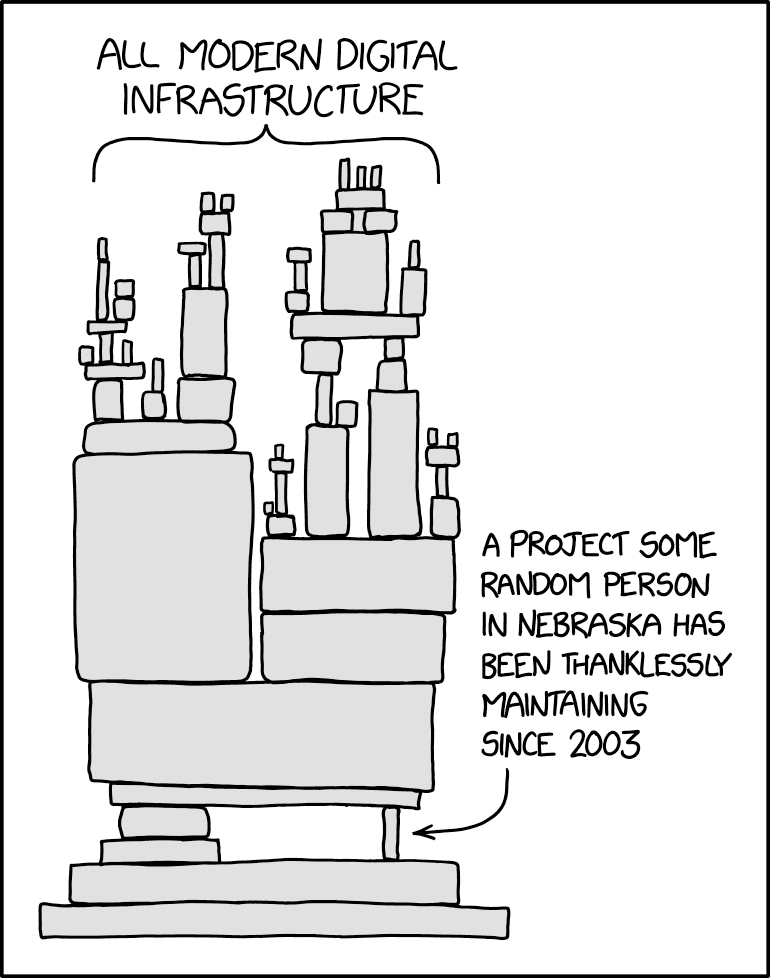
\includegraphics[width=0.5\textwidth]{images/2347.png}\end{center}

which does \textit{not} contain the phrase ``the most consequential figures in the tech world''. As it happens, it \textit{also} doesn't contain the phrase ``ronald's universal number kounter'', which instead comes from @6thgradeforever's tweet.

\section{Quick Start: Getting Something To Happen}

Open ``dunk.circ'' in logisim. There you will see the various components, and wires between them. The quickest way to get something to happen is to load one of the example binaries from the folder ``examples/bin'' into memory and turn on auto-tick. To do this, right-click on the RAM unit (top right) and select ``Load Image...'';

    \begin{center}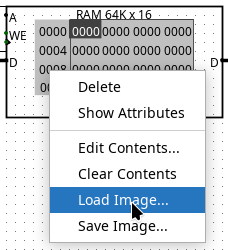
\includegraphics[width=0.25\textwidth]{images/load_image.png}\end{center}

Then navigate to and select one of the assembled examples under examples/bin. You can then manually tick the clock with the hotkey ``Ctrl+T'', or you begin automatic ticking with ``Ctrl+K'' or selecting ``Auto-Tick Enabled'' under the ``Simulate'' menu. The simulation should then begin, and the CPU will run the code. The speed of Auto-Tick can be changed under the ``Simulate'' menu; I recommend cranking it up. Try running the binary \Verb|examples/bin/hello_world|. I'm sure you'll be surprised by what happens.

\section{The Instruction Set And Assembler}

Dunk uses an instruction set comparable to a slimmed-down version of the x86 instruction set. Associated with dunk is the assembler ``dunkasm'', which compiles dunk assembly files into runnable machine code\footnote{Due to a quirk in Logisim's interface, to avoid unnecessary clicking, I have set the compiler to, by default, output the binaries in "v3 hex words addressed" format, which is actually a text file containing the binary code in hex format. It can produce raw binary via the \Verb|-b| flag.}. The assembly language features some quality-of-life improvements over the typical assembly language, as I don't expect there to ever exist a compiler for a high-level language for dunk (at least, not the logisim version), so I wanted to make the assembly language pleasant to use. A fairly immediate example of this is the \textit{human-readability} of instructions. For instance, in place of something like ``\Verb|bgez|'', as in the RISC-V instruction set RV32I, I named my analogue ``\Verb{goto_if_nonnegative}''. The other main QOL feature is \textit{aliases}. The commands ``alias'' and ``dealias'' allow one to define and undefine aliases; for instance, the command \Verb|alias x r0| defines an alias ``\Verb|x|'', instances of which the assembler will replace with the string ``r0''. Instructions, registers, memory addresses and constants can all be given aliases. The specific behaviour of syntax rules for aliases will be detailed elsewhere in the docs. The assembler also has inbuilt aliases, such as, for instance, the alises ``argument1''-``argument9'', where \Verb|argumentN|, for \Verb|N| from 1-9, is replaced by \Verb|r[8+N-1]|, which are general-purpose registers, but, by convention, used to pass arguments to functions\footnote{This can also be done using the stack, but the relative positionof the stack after a \Verb|call| is not consistent; see the section on preservation of registers}. To see this in action, consider the following code snipped, defining a simple function to compute the remainder of an integer on division by another.

\begin{BVerbatim}


    alias x r0
    alias y r1

    remainder:
        set x argument1
        set y argument2
        
        remainder_loop:
	        subtract x y
	        
	        goto_if_negative x remainder_done
	        
	        goto remainder_loop
        
        remainder_done:
	        add x y
	        set result1 x
	        return
	        
	        
\end{BVerbatim}

The calling code can then access the result in the register \Verb|argument1|, since \Verb|x| is \Verb|argument1|, which is modified in place. Additionally, there is a built-in alias \Verb|result1| which also refers to \Verb|r8|, purely to allow the user to distinguish between when \Verb|r8| is being used to pass as argument, or as a return value.

Another example of the qualilty-of-life features of the dunk assembly language can be seen in the hello world example source, \Verb|examples/src/hello_world.dasm|: it consists of the single line

\begin{BVerbatim}


	prints "Hello, world!" PRINT_ADDR


\end{BVerbatim}

Here we see the inbuilt string-printing intruction, which supplies the address of a byte-string to the string-printing unit connected to the terminal, which accesses the memory directly. In earlier iterations, I sent characters one-by-one to the terminal via a hand-written function, but this was very slow, considering logisim's simulation would max out at around 30Hz (a far cry from the >2GHz seen in modern hardware), so I build the string-printing unit to send a character to the terminal at each clock-edge, until a null terminator is encountered. We also see that string literals are presented inline; the assembler stores the literals in the strings section of the produced binary, which follows the code, and inserts the address of the string in place of the string literal in the code. Therefore one can write a ``hello world'' that looks not dissimilar to a line one might encounter in python. Trailing the string is \Verb|PRINT_ADDR|, which is an alias for \Verb|0xfffc|, which is the address of the memory-mapped write-only register connected to the string-printing unit.

\newpage
\section{Architecture; How DUNK Works}

Dunk has four main buses: the two control buses, the data bus, and the address bus. The control buses run in parallel, issuing microcode instructions to the units. These are decoded internally by each unit into signals determining how the unit will transform its internal state or output data onto any buses. The two buses allow dunk to execute up to two opcodes at a time, allowing for a degree of parallelism, which improves performance. The data bus is used to send general-purpose data between units, and the address bus is used to address memory. The buses are controlled by registers; each clock cycle, the control buses are updated to output the current output of the control bus, and the data bus updates to output what ever is being sent to it by any of the various units, and similarly for the address bus. The control and data buses are updated on the rising edge of the clock, while the address bus is updated on the falling edge, to allow memory read microcodes to be issued during the same clock cycle as memory addresses are sent to the address bus. There are additional microcode instructions to prevent the data and address buses from being updated, or for one to assume the value of the other.

Inside dunk's control unit, there are three ROMs. One is the decoder ROM, and the other two are microcode ROMs. The decoder ROM is fed the opcode of an instruction fetched from memory, and inputs this as the address into the decoder ROM. The data stored at this address is the address of the microcode for executing that instruction in the microcode ROMS. This is then stored in a register, the ``\Verb|MAR|'', for micro-code address register, which sends its value to the address input of the two microcode ROMs. The values stored in the microcode ROMS are then altered by the ``microcode mixer'', which inserts any necessary parameters\footnote{Which parameters - and where they can be fetched from - is encoded in the microcodes themselves. Typically, they are stored in the upper byte of the instruction, or an ``overflow word'' following the instruction in memory}, and then sent out on to the control buses, which control the other units. Every clock cycle, unless stalled, \Verb|MAR| is incremented, progressing to the next micro-operation, until it encounters the ``\Verb|done|'' microcode, which immediately resets \Verb|MAR| to 0. It then continues incrementing; The first two words in the microcode ROMs contain microcode that fetches the next instruction from main memory, beginning the cycle over again.

The contents of these ROMs, additionally the ROM for the real-time disassembler, are generated by the dunk programmer, which can be found under utils/dunkprog. In utils/dunkprog/include one can find header files defining the instruction opcodes (\Verb|opcodes.h|) and the microcodes (\Verb|microops.h|). The main file \Verb|utils/dunkprog/src/dunkprog.c| contains the microcode sequences for the instructions.

\subsection{The Units}

Dunk contains 5 main units, which may be seen laid out accross the top of the schematic; the control unit, which issues microcode instructions, the registers unit, which contains the 16 general-purpose registers, the arithmetic logic unit, which performs arithmetic and logic operations, the \textit{special} registers unit, which contains registers with specific purposes and non-standard behaviour, and the memory controller, which handles the reading and writing of main memory, as well as memory-mapped I/O. The leftmost unit, reading ``instr disp'', is the real-time disassembler/debugger, which prints instructions, as they are executed, in the syntax of dunk assembly. This unit does not affect the functioning of the CPU, and may be turned off using the attached button. It features a specialised ``micro-clocked'' architecture, which will be discussed in another section.

\subsubsection{The Control Unit}

\subsubsection{The Register Unit}

\subsubsection{The Special Register Unit}

\subsubsection{The Arithmetic Logic Unit}

\subsubsection{The Memory Controller}

\section{The Real-Time Disassembler}

The real-time disassembler presents the assembly code (sans aliases) of the current instruction being run. To achieve this, I needed to produce ASCII strings of variable length, actively decoded at runtime, with parameters inserted, in a human-readable format, in a way that can be displayed instantaneously inside logisim. This is not possible. Indeed, the terminal to which it is connected only accepts \textit{one} ASCII character per rising-edge of the clock. So, how does it work? It takes advantage of a quirk of logisim's simulation model. Consider the following schematic.

	\begin{center}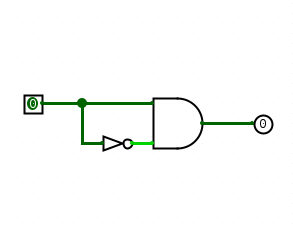
\includegraphics[width=0.25\textwidth]{images/and_not.png}\end{center}

A logical analysis of this circuit shows that it always outputs a logical 0. Indeed, in formal logic notation, $p \land \neg p = \bot$ for any $p$. However logisim doesn't use any internal formal logic algebra; rather, it computes the values in ``propagation steps''. Under the \Verb|Simulate| menu, one can disable auto-propagate, and step through the propagation steps with \Verb|Single-Step Propagation|;

	\begin{center}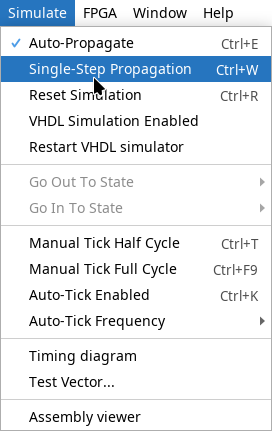
\includegraphics[width=0.25\textwidth]{images/single_step.png}\end{center}

In doing so, one can observe the following. If the input pin in the above schematic is set to 1, a single propagation set propagates this value along the wires leading to the \gate{and} and \gate{not} gates. A second propagation step, and the \gate{and} and \gate{not} gates change their output according to their \textit{current} inputs. The \gate{and} gate is currently recieving a 1 from the pin, and a 1 from the \gate{not} gate which, are the time of the propatation step, has not yet updated its output. Therefore, the \gate{and} gate outputs a 1;

	\begin{center}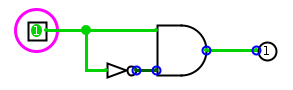
\includegraphics[width=0.25\textwidth]{images/spurious_1.png}\end{center}

Another propagation step, and the \gate{and} gate updates its value according to the newly low input coming from the \gate{not} gate. As a result, the output of the circuit is not constant 0, but very, very briefly, 1. This is a real effect; a physical implementation of the above circuit will display a brief bump when the input changes from low to high. However, this effect cannot be taken advantage of; the duration, voltage, etc of this bump varies with environmental factors such as temperature and humidity, and so any circuits intentionally using this effect to achieve an outcome will be unreliable, and will exhibit unpredictable metastability. However, in logisim, this \textit{is} reliable. If the above circuit is connected to the clock input of a D-flip flop, \textit{it will be updated whenever the input to the \gate{and} gate rises}.

	\begin{center}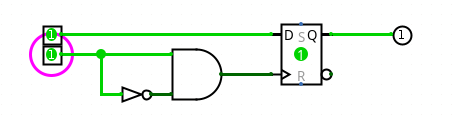
\includegraphics[width=0.5\textwidth]{images/spurious_clock.png}\end{center}

\end{document}
